%TCIDATA{LaTeXparent=0,0,cap_RevisaoBibliografica.tex}

\section{M\'{e}todos Convencionais de Recupera\c{c}\~{a}o Secund\'{a}ria}

\subsection{Conceito e Contextualiza\c{c}\~{a}o da Recupera\c{c}\~{a}o Secund\'{a}ria}

De acordo com Rosa, nas acumula\c{c}\~{o}es de petr\'{o}leo h\'{a}, na \'{e}poca de sua descoberta, uma dada quantidade de energia, chamada de \textit{energia prim\'{a}ria}, cuja grandeza \'{e} determinada pelo volume e pela natureza dos fluidos existentes no meio, al\'{e}m dos n\'{i}veis de press\~{a}o e temperatura do reservat\'{o}rio; a quantidade de \'{o}leo retirada utilizando-se unicamente a energia do reservat\'{o}rio \'{e} denominada \textit{recupera\c{c}\~{a}o prim\'{a}ria} \cite{engres}. Haynes \textit{et al.} citam algumas formas de recupera\c{c}\~{a}o prim\'{a}ria, tais como: g\'{a}s em solu\c{c}\~{a}o, expans\~{a}o de g\'{a}s livre, influxo natural de \'{a}gua ou for\c{c}a gravitacional; os autores afirmam que a efici\^{e}ncia de recupera\c{c}\~{a}o prim\'{a}ria \'{e} menor nos processos envolvendo gases, maior em processos envolvendo \'{a}gua e gravita\c{c}\~{a}o, este \'{u}ltimo respons\'{a}vel pelos melhores resultados \cite{oil1976}.

Quando se d\'{a} o processo de produ\c{c}\~{a}o, parte da energia prim\'{a}ria \'{e} dissipada por causa da descompress\~{a}o dos fluidos do reservat\'{o}rio e das resist\^{e}ncias que os mesmos encontram ao fluir em dire\c{c}\~{a}o aos po\c{c}os produtores --- resist\^{e}ncias associadas \`{a}s for\c{c}as viscosas e capilares presentes no meio poroso \cite{engres}. Alotaibi afirma que essa energia \'{e} rapidamente depletada; a consequ\^{e}ncia dessa dissipa\c{c}\~{a}o de energia prim\'{a}ria resulta no decr\'{e}scimo de press\~{a}o do reservat\'{o}rio em sua vida produtiva e, consequentemente, na redu\c{c}\~{a}o da produtividade dos po\c{c}os \cite{alotaibi}. 

De forma a se minorar os efeitos danosos da dissipa\c{c}\~{a}o da energia prim\'{a}ria, existem duas linhas de a\c{c}\~{a}o a serem consideradas:

\begin{itemize}
\item Reduzir as resist\^{e}ncias viscosas e/ou capilares por meio de m\'{e}todos especiais, como por exemplo aquecendo a jazida;
\item Adicionar suplemento de energia secund\'{a}ria, artificialmente comunicada, atrav\'{e}s de inje\c{c}\~{a}o de fluidos em po\c{c}os selecionados.
\end{itemize}

Quando se suplementa o reservat\'{o}rio com energia transferida artificialmente, ou se empregam meios de incrementar a efici\^{e}ncia da energia prim\'{a}ria, a quantidade adicional de \'{o}leo produzida \'{e} chamada de \textit{recupera\c{c}\~{a}o secund\'{a}ria}. Por extens\~{a}o, todas as opera\c{c}\~{o}es que conduzem \`{a} obten\c{c}\~{a}o desse adicional de \'{o}leo tamb\'{e}m s\~{a}o denominadas recupera\c{c}\~{a}o secund\'{a}ria. Essas opera\c{c}\~{o}es, atualmente, s\~{a}o implantadas em sua grande maioria o t\~{a}o cedo quanto poss\'{i}vel na vida do reservat\'{o}rio.

\'{E} importante ressaltar que h\'{a} uma diferen\c{c}a entre recupera\c{c}\~{a}o secund\'{a}ria e m\'{e}todos de eleva\c{c}\~{a}o artificial e de estimula\c{c}\~{a}o de po\c{c}os; estes n\~{a}o afetam diretamente as energias expulsivas do reservat\'{o}rio, embora sua aplica\c{c}\~{a}o concorra para economiz\'{a}-las. As t\'{e}cnicas de eleva\c{c}\~{a}o artificial\footnote{Ver \cite{engpetro}.} e de estimula\c{c}\~{a}o de po\c{c}os est\~{a}o mais ligadas ao comportamento dos po\c{c}os produtores do que ao comportamento do reservat\'{o}rio como um todo. Contudo, a linha divis\'{o}ria entre tais m\'{e}todos e os m\'{e}todos de recupera\c{c}\~{a}o secund\'{a}ria n\~{a}o \'{e} muito n\'{i}tida --- certos m\'{e}todos de estimula\c{c}\~{a}o, como a inje\c{c}\~{a}o c\'{i}clica de vapor, s\~{a}o usualmente inclu\'{i}dos entre os m\'{e}todos de recupera\c{c}\~{a}o secund\'{a}ria \cite{engres}.

Ainda segundo Rosa, h\'{a} dois objetivos pr\'{a}ticos b\'{a}sicos dos m\'{e}todos de recupera\c{c}\~{a}o secund\'{a}ria:

\begin{itemize}
\item \textbf{Aumento da efici\^{e}ncia de recupera\c{c}\~{a}o} --- A efici\^{e}ncia de recupera\c{c}\~{a}o prim\'{a}ria \'{e} normalmente baixa; em alguns casos, dependendo das caracter\'{i}sticas do reservat\'{o}rio e dos fluidos, ela pode ser at\'{e} nula. Em alguns casos, a efici\^{e}ncia de recupera\c{c}\~{a}o secund\'{a}ria pode passar de 60\% em casos bem-sucedidos; contudo, o valor mais frequente dessa efici\^{e}ncia, nos m\'{e}todos convencionais, se situa entre 30 e 50\%.
\item \textbf{Acelera\c{c}\~{a}o da produ\c{c}\~{a}o} --- O emprego dos m\'{e}todos de recupera\c{c}\~{a}o secund\'{a}ria busca acelerar a produ\c{c}\~{a}o ou ao menos reduzir a taxa de seu decl\'{i}nio natural. A acelera\c{c}\~{a}o da produ\c{c}\~{a}o resulta em antecipa\c{c}\~{a}o do fluxo de caixa; portanto, h\'{a} o aumento de seu valor presente e uma consequente melhoria da economicidade da explora\c{c}\~{a}o do campo ou reservat\'{o}rio.
\end{itemize}

Al\'{e}m dos objetivos b\'{a}sicos de emprego da recupera\c{c}\~{a}o secund\'{a}ria, ha v\'{a}rios outros incentivos ao uso desses m\'{e}todos, tais como: pre\c{c}o do petr\'{o}leo; custos de explora\c{c}\~{a}o, desenvolvimento e produ\c{c}\~{a}o; e avan\c{c}os tecnol\'{o}gicos na \'{a}rea. Por\'{e}m, destaca-se que apenas o uso dessas t\'{e}cnicas n\~{a}o \'{e} o suficiente para mitigar todos os males da produ\c{c}\~{a}o de petr\'{o}leo e do esgotamento das reservas; outras medidas podem e devem ser tomadas, simultaneamente, para aumentar a efici\^{e}ncia e a rentabilidade da produ\c{c}\~{a}o, tais como\footnote{Ver \cite{engres}}:
%TODO encontrar as paginas do Rosa para essa parte
\begin{itemize}
\item \textbf{Explora\c{c}\~{a}o de reservas n\~{a}o convencionais} --- Xistos e folhelhos betuminosos, por exemplo, acumulam grandes quantidades de \'{o}leo. V\'{a}rias dessas reservas j\'{a} foram encontradas em regi\~{o}es como Athabasca, no Canad\'{a}, cintur\~{a}o do Orinoco, na Venezuela, e o Colorado, nos Estados Unidos. O custo de produ\c{c}\~{a}o nessas reservas \'{e} consider\'{a}vel, mas j\'{a} se projetam meios tecnol\'{o}gicos para reduzir o mesmo. Entre outras reservas n\~{a}o convencionais de hidrocarbonetos, h\'{a} a presen\c{c}a de g\'{a}s natural em solu\c{c}\~{a}o existente na \'{a}gua de aqu\'{i}feros; embora a raz\~{a}o de solubilidade do g\'{a}s natural na \'{a}gua normalmente seja pequena, o imenso volume dos aqu\'{i}feros perimitiria uma produ\c{c}\~{a}o de grandes volumes desse g\'{a}s. Uma outra reserva n\~{a}o convecional poder\'{a} ser o g\'{a}s natural proveniente de hidratos localizados no fundo de oceanos e em regi\~{o}es congeladas da Terra.
\item \textbf{Estimula\c{c}\~{a}o de Po\c{c}os} De acordo com Thomas, a estimula\c{c}\~{a}o de po\c{c}os \'{e} um conjunto de atividades realizadas com o objetivo de aumentar o \'{i}ndice de produtividade ou injetividade do po\c{c}o \cite[p.~166]{engpetro}. Os principais m\'{e}todos de estimula\c{c}\~{a}o s\~{a}o: fraturamento hidr\'{a}ulico, em que se cria, atrav\'{e}s de uma ruptura na rocha-reservat\'{o}rio causada por um elevado gradiente de press\~{a}o, um caminho preferencial de alta condutividade, facilitando um fluxo de fluidos do reservat\'{o}rio ao po\c{c}o (ou vice-versa); e acidifica\c{c}\~{a}o, onde se injeta um \'{a}cido com press\~{a}o inferior \`{a} press\~{a}o de fraturamento da forma\c{c}\~{a}o, visando remover danos da mesma. Tais m\'{e}todos contribuem para a acelera\c{c}\~{a}o da produ\c{c}\~{a}o e at\'{e}, em alguns casos, o aumento da efici\^{e}ncia de recupera\c{c}\~{a}o. A aplica\c{c}\~{a}o de m\'{e}todos de estimula\c{c}\~{a}o pode, inclusive, ser feita em campos submetidos a opera\c{c}\~{o}es de recupera\c{c}\~{a}o secund\'{a}ria.
\item \textbf{Uso de po\c{c}os especiais} --- Nas \'{u}ltimas d\'{e}cadas houve um incremento consider\'{a}vel no uso dos chamados \textit{po\c{c}os especiais}, que possuem como caracter\'{i}stica marcante a n\~{a}o-verticalidade, Segundo Thomas, esses po\c{c}os s\~{a}o perfurados com v\'{a}rias finalidades, como: controlar um po\c{c}o em \textit{blowout} por meio de po\c{c}os de al\'{i}vio; atingir forma\c{c}\~{o}es produtoras abaixo de locais inacess\'{i}veis, como rios, lagos, cidades, entre outros; desviar a trajet\'{o}ria do po\c{c}o de acidentes geol\'{o}gicos, como domos salinos e falhas; perfurar v\'{a}rios po\c{c}os de um mesmo ponto, como \'{e} o caso da produ\c{c}\~{a}o em plataformas mar\'{i}timas; e desviar po\c{c}os que tiveram seu trecho final perdido por problemas operacionais \cite[p. 106]{engpetro}. O uso desses po\c{c}os inclinados, horizontais, multilaterais, etc., pode aumentar a velocidade de drenagem do reservat\'{o}rio, ou seja, antecipar a produ\c{c}\~{a}o, bem como aumentar a efici\^{e}ncia de recupera\c{c}\~{a}o atrav\'{e}s do aumento da efici\^{e}ncia de varrido, por exemplo.
\item \textbf{Extra\c{c}\~{a}o de l\'{i}quidos de g\'{a}s natural} --- A produ\c{c}\~{a}o de hidrocarbonetos l\'{i}quidos pode ser aumentada pela instala\c{c}\~{a}o de plantas de gasolina natural e de unidades port\'{a}teis de extra\c{c}\~{a}o de l\'{i}quidos de g\'{a}s natural.
\item \textbf{Reestudo de \'{a}reas julgadas improdutivas ou antiecon\^{o}micas} --- Mesmo que as reservas mundiais de petr\'{o}leo sejam limitadas, elas est\~{a}o longe de terem sido totalmente exploradas; de fato, apenas uma pequena porcentagem da superf\'{i}cie do planeta foi inteiramente explorada. Seja na terra ou no fundo do mar, h\'{a} ainda perspectivas not\'{a}veis fora das \'{a}reas hoje em produ\c{c}\~{a}o; al\'{e}m disso, as estimativas do volume de \'{o}leo que ainda poder\'{a} ser descoberto s\~{a}o ainda vagas. \'{E} com essa perspectiva que a ind\'{u}stria pode medir as oportunidades que tem \`{a} frente no caso de esgotamento das \'{a}reas hoje em produ\c{c}\~{a}o. Portanto, de um modo geral, deve-se pensar sempre na ado\c{c}\~{a}o das seguintes medidas, sem danos ao andamento das opera\c{c}\~{o}es de recupera\c{c}\~{a}o secund\'{a}ria: estudar novas \'{a}reas; estudar forma\c{c}\~{o}es mais profundas (o pr\'{e}-sal \'{e} um exemplo); reestudar \'{a}reas consideradas esgotadas ou de produ\c{c}\~{a}o antiecon\^{o}mica; e investir mais dinheiro, tempo e pessoal em treinamento e pesquisa, visando melhorar os m\'{e}todos de explora\c{c}\~{a}o e produ\c{c}\~{a}o existentes.
\end{itemize}

\subsection{Classifica\c{c}\~{a}o dos M\'{e}todos de Recupera\c{c}\~{a}o Secund\'{a}ria}
Segundo Rosa, os m\'{e}todos de recupera\c{c}\~{a}o de \'{o}leo visando suplementar a energia do reservat\'{o}rio, logo ap\'{o}s a fase de recupera\c{c}\~{a}o prim\'{a}ria, eram denominados, originalmente, m\'{e}todos de recupera\c{c}\~{a}o secund\'{a}ria, enquanto que m\'{e}todos empregados posteriormente passaram a ser chamados de \textit{recupera\c{c}\~{a}o terci\'{a}ria}; Alotaibi afirma que os m\'{e}todos de recupera\c{c}\~{a}o terci\'{a}ria s\~{a}o utilizados para se recuperar \'{o}leo residual logo ap\'{o}s o emprego de t\'{e}cnicas como a inje\c{c}\~{a}o de \'{a}gua \cite{alotaibi}. Adeniyi \textit{et al.} afirmam que a recupera\c{c}\~{a}o terci\'{a}ria reduz a viscosidade do \'{o}leo para incrementar sua produ\c{c}\~{a}o; os autores destacam que tais m\'{e}todos tamb\'{e}m podem ser utilizados caso haja componentes de \'{o}leo cru pesado \cite{adeniyi2008}. 

Os m\'{e}todos tamb\'{e}m podiam ser classificados de acordo com a sua cronologia de aplica\c{c}\~{a}o em determinado campo ou reservat\'{o}rio. Posteriormente, todos os m\'{e}todos de recupera\c{c}\~{a}o aplicados com o objetivo de aumentar a efici\^{e}ncia de recupera\c{c}\~{a}o e/ou acelerar a produ\c{c}\~{a}o em rela\c{c}\~{a}o \`{a} produ\c{c}\~{a}o prim\'{a}ria passaram a ser denominados de recupera\c{c}\~{a}o secund\'{a}ria.

Nas \'{u}ltimas d\'{e}cadas, a classifica\c{c}\~{a}o dos m\'{e}todos de recupera\c{c}\~{a}o secund\'{a}ria se deu em \textit{m\'{e}todos convencionais} (os antigos m\'{e}todos de recupera\c{c}\~{a}o secund\'{a}ria) e \textit{m\'{e}todos especiais} (os antigos m\'{e}todos de recupera\c{c}\~{a}o terci\'{a}ria), os \'{u}ltimos tamb\'{e}m conhecidos, na literatura inglesa, como m\'{e}todos de \textit{EOR} (\textit{Enhanced Oil Recovery}) --- esse termo, nos \'{u}ltimos anos, tem sido substitu\'{i}do pelo termo \textit{IOR} (\textit{Improved Oil Recovery}), cuja diferen\c{c}a, em rela\c{c}\~{a}o ao \textit{EOR}, reside no fato de que os m\'{e}todos de \textit{IOR} englobam, al\'{e}m dos m\'{e}todos de \textit{EOR}, quaisquer m\'{e}todos ou t\'{e}cnicas n\~{a}o-convencionais ou modernas que possuam o objetivo de aumentar a produ\c{c}\~{a}o e/ou acelerar a produ\c{c}\~{a}o em rela\c{c}\~{a}o \`{a} produ\c{c}\~{a}o prim\'{a}ria e/ou secund\'{a}ria \cite[p. 564]{engres}. 

O estudo das t\'{e}cnicas de EOR concentrou esfor\c{c}os de v\'{a}rios pesquisadores, desde a d\'{e}cada de 1970, em que tais m\'{e}todos se tornaram populares \cite{coats1982}; Udy \textit{et al.} destacam o uso dessas t\'{e}cnicas acopladas a m\'{e}todos de otimiza\c{c}\~{a}o para se tentar maximizar a produ\c{c}\~{a}o de petr\'{o}leo \cite{udyEOR}; Ling \textit{et al.} analisam a implementa\c{c}\~{a}o e o efeito de v\'{a}rias t\'{e}cnicas de EOR na Forma\c{c}\~{a}o de Bakken, situada na Depress\~{a}o de Williston, EUA, de maneira a se utilizar o melhor m\'{e}todo na quest\~{a}o da recupera\c{c}\~{a}o de \'{o}leo \cite{ling2014}; Alvarado e Manrique apresentam a evolu\c{c}\~{a}o de alguns m\'{e}todos de EOR ao longo dos anos, e afirmam que as t\'{e}cnicas de IOR, al\'{e}m de emcompassarem as de EOR, incluem novas tecnologias de perfura\c{c}\~{a}o e de po\c{c}os, administra\c{c}\~{a}o e controle inteligente de reservat\'{o}rios, t\'{e}cnicas de monitoramento avan\c{c}ado de reservat\'{o}rios, al\'{e}m de aplica\c{c}\~{o}es de diferentes melhorias de processos de recupera\c{c}\~{a}o prim\'{a}ria e secund\'{a}ria \cite{alvarado2010}.

Em termos da classifica\c{c}\~{a}o mais atual, s\~{a}o m\'{e}todos convencionais de recupera\c{c}\~{a}o secund\'{a}ria os m\'{e}todos de inje\c{c}\~{a}o de \'{a}gua e inje\c{c}\~{a}o imisc\'{i}vel de g\'{a}s. J\'{a} os m\'{e}todos especiais incluem, entre outros, a inje\c{c}\~{a}o misc\'{i}vel de g\'{a}s, a inje\c{c}\~{a}o de vapor, a inje\c{c}\~{a}o de pol\'{i}meros e a combust\~{a}o \textit{in situ}\footnote{Tais m\'{e}todos s\~{a}o citados em \cite{oil1976}. Uma abordagem sobre os m\'{e}todos especiais pode ser encontrada em \cite[pp. 677-726]{engres}}. A Figura \ref{fig:recreview} destaca os m\'{e}todos mais comuns de recupera\c{c}\~{a}o.

\begin{figure}[!ht]
	\centering
	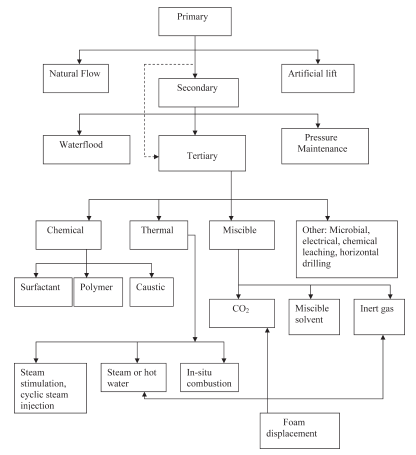
\includegraphics[width=.6\textwidth]{figs/revisao/revisao_recmethods}
	\caption{Resumo dos m\'{e}todos convencionais de recupera\c{c}\~{a}o \cite{adeniyi2008} \label{fig:recreview}}
\end{figure}

\subsection{M\'{e}todos Convencionais}
Os dois tipos de m\'{e}todos considerados convencionais, j\'{a} citados, s\~{a}o os m\'{e}todos de inje\c{c}\~{a}o imisc\'{i}vel de fluidos no reservat\'{o}rio, seja \'{a}gua ou g\'{a}s. Segundo Eremin, o m\'{e}todo de inje\c{c}\~{a}o de \'{a}gua \'{e} um dos mais utilizados devido \`{a} sua utiliza\c{c}\~{a}o tamb\'{e}m como m\'{e}todo mantenedor da press\~{a}o no reservat\'{o}rio, al\'{e}m do fato da \'{a}gua ser um fluido acess\'{i}vel, consideravelmente barato e possuir propriedade de deslocamento espec\'{i}fica \cite{eremin}. J\'{a} a inje\c{c}\~{a}o de imisc\'{i}vel de g\'{a}s consiste em inje\c{c}\~{a}o de fluido gasoso, mas de forma que ele n\~{a}o se misture ao \'{o}leo, criando uma mistura bif\'{a}sica \cite[p. 564]{engres}.

O uso de m\'{e}todos convencionais, como o de inje\c{c}\~{a}o de \'{a}gua, \'{e} antigo dentro da hist\'{o}ria da explora\c{c}\~{a}o do petr\'{o}leo; se considera que o primeiro caso de inje\c{c}\~{a}o de \'{a}gua ocorreu acidentalmente na Pensilv\^{a}nia, em 1865. Em 1880, se descobriu que a \'{a}gua, ao invadir os po\c{c}os por meio de areias rasas, contribu\'{i}a para um aumento na recupera\c{c}\~{a}o de \'{o}leo. Muitas das primeiras ocorr\^{e}ncias de invas\~{a}o de \'{a}gua nos reservat\'{o}rios eram acidentais, decorrentes de \'{a}guas provenientes de areias \'{u}midas ou da superf\'{i}cie invadindo os po\c{c}os e, consequentemente, o reservat\'{o}rio \cite{adeniyi2008}. A partir de 1950, afirmam Singh e Kiel, as t\'{e}cnicas de inje\c{c}\~{a}o de \'{a}gua se tornaram mais populares, sua utiliza\c{c}\~{a}o incrementando rapidamente. Atualmente, a inje\c{c}\~{a}o de \'{a}gua \'{e} ainda considerada como um dos m\'{e}todos de recupera\c{c}\~{a}o mais confi\'{a}veis e econ\^{o}micos, a ponto de se tornar a alternativa a ser usada em caso de deple\c{c}\~{a}o de reservat\'{o}rios cujo mecanismo \'{e} o influxo de \'{a}gua \cite{singh1982}.

Segundo Rosa, ao se escolher um projeto de inje\c{c}\~{a}o, deve-se levar em conta a escolha do esquema de inje\c{c}\~{a}o, isto \'{e}, da distribui\c{c}\~{a}o dos po\c{c}os de inje\c{c}\~{a}o e de produ\c{c}\~{a}o mais adequada ao reservat\'{o}rio de petr\'{o}leo em estudo. Como o objetivo primordial da inje\c{c}\~{a}o \'{e} o aumento da recupera\c{c}\~{a}o de petr\'{o}leo, deve-se tentar produzir esse volume adicional desejado utilizando-se esquemas em que os volumes de fluidos injetados sejam os menores poss\'{i}veis e a produ\c{c}\~{a}o do fluido injetado seja a menor poss\'{i}vel. Por fim, devem ser observadas as caracter\'{i}sticas particulares do reservat\'{o}rio em estudo, como a exist\^{e}ncia de falhas, varia\c{c}\~{o}es de permeabilidade, etc., al\'{e}m do aspecto econ\^{o}mico da produ\c{c}\~{a}o \cite[p. 564]{engres}; o aspecto econ\^{o}mico envolve estudo de custos relacionados \`{a} ado\c{c}\~{a}o do m\'{e}todo de recupera\c{c}\~{a}o, como os custos de estudo, de perfura\c{c}\~{a}o de novos po\c{c}os, da convers\~{a}o de po\c{c}os produtores em injetores, entre outros \cite{latil}.

De acordo com Latil, entre os m\'{e}todos convencionais de inje\c{c}\~{a}o de fluidos, o de inje\c{c}\~{a}o de g\'{a}s \'{e} mais indicado em casos de reservat\'{o}rios com baixa raz\~{a}o g\'{a}s-\'{o}leo --- neste caso, seria necess\'{a}ria um grande volume de g\'{a}s injetado para se criar a fase gasosa --- ou de \'{o}leo saturado, desde que a permeabilidade \`{a} \'{a}gua seja suficientemente alta; j\'{a} em casos de reservat\'{o}rios com alta raz\~{a}o gas-\'{o}leo, a inje\c{c}\~{a}o imisc\'{i}vel de g\'{a}s se torna um m\'{e}todo que resulta em melhores \'{i}ndices de recupera\c{c}\~{a}o de \'{o}leo. Por fim, em casos de reservat\'{o}rios heterog\^{e}neos com presen\c{c}a de \'{a}gua, a inje\c{c}\~{a}o de \'{a}gua \'{e} a mais recomendada \cite{latil}. 

\subsection{Esquemas de Inje\c{c}\~{a}o}

Ao se considerar o uso de t\'{e}cnicas de recupera\c{c}\~{a}o secund\'{a}ria, baseadas na inje\c{c}\~{a}o de fluidos, a efici\^{e}ncia do m\'{e}todo utilizado depende da maneira com que os po\c{c}os injetores e produtores s\~{a}o posicionados. A disposi\c{c}\~{a}o dos mesmos no reservat\'{o}rio deve ser tal que minimize o n\'{u}mero de po\c{c}os, mas maximizando a inje\c{c}\~{a}o de fluido e melhorando a recupera\c{c}\~{a}o de \'{o}leo \cite{dake}. O posicionamento dos po\c{c}os pode ser encarado como um \textit{esquema de inje\c{c}\~{a}o}. Segundo Rosa, h\'{a} v\'{a}rios tipos de esquemas de inje\c{c}\~{a}o, separados em dois grupos principais: os esquemas baseados na estrutura do reservat\'{o}rio (inje\c{c}\~{a}o perif\'{e}rica, no topo ou na base) ou baseados no modo como os po\c{c}os s\~{a}o distribu\'{i}dos (esquemas em malha) \cite[p. 564]{engres}.

\subsubsection{Esquemas baseados na Estrutura do Reservat\'{o}rio}
Nos esquemas baseados na estrutura do reservat\'{o}rio, os po\c{c}os de mesmo tipo (de inje\c{c}\~{a}o ou de produ\c{c}\~{a}o) se concentram em determinadas \'{a}reas do reservat\'{o}rio. Em reservat\'{o}rios de estrutura anticlinal, por exemplo, \'{e} mais utilizado o esquema de \textit{inje\c{c}\~{a}o perif\'{e}rica}, em que os po\c{c}os produtores se concentram no centro do reservat\'{o}rio, equanto que os injetores s\~{a}o situados na periferia do mesmo, justificando o nome do esquema\footnote{Ver \cite[p. 565]{engres}}. O esquema de inje\c{c}\~{a}o perif\'{e}rica pode ser aplicado juntamente com projetos de otimiza\c{c}\~{a}o dos injetores, como por exemplo o problema real abordado por Feng \textit{et al.}, tratando-se de um problema de \textit{design} de um projeto \'{o}timo de inje\c{c}\~{a}o de \'{a}gua em um campo de petr\'{o}leo situado no Equador \cite{feng2015}. 

A \textit{inje\c{c}\~{a}o no topo} consiste em situar os po\c{c}os injetores no topo do reservat\'{o}rio, enquanto os produtores s\~{a}o localizados na base; o fluido injetado, neste caso, \'{e} o g\'{a}s. Por fim, a \textit{inje\c{c}\~{a}o na base} considera os po\c{c}os injetores na base do reservat\'{o}rio e os produtores no topo, com a \'{a}gua sendo o fluido injetado. Vale notar que os esquemas de inje\c{c}\~{a}o no topo e na base podem ser combinados, e que, em determinado momento, os po\c{c}os produtores podem ser convertidos em po\c{c}os injetores. Rosa ainda destaca que, na verdade, essas diferentes maneiras de se fazer inje\c{c}\~{a}o n\~{a}o se classificam exatamente como
\textit{esquemas} de inje\c{c}\~{a}o, uma vez que a disposi\c{c}\~{a}o dos po\c{c}os n\~{a}o est\'{a} previamente estabelecida, ou seja, n\~{a}o existem arranjos prefixados para a localiza\c{c}\~{a}o dos po\c{c}os \cite[p. 566]{engres}.


Um fato a ser considerado com a inje\c{c}\~{a}o de \'{a}gua, afirma Patacchini, \'{e} que n\~{a}o \'{e} poss\'{i}vel simplemente adicionar a referida vari\'{a}vel \`{a}s equa\c{c}\~{o}es de balan\c{c}o de materiais em projetos de inje\c{c}\~{a}o perif\'{e}rica, uma vez que as equa\c{c}\~{o}es n\~{a}o consideram o volume de \'{a}gua perdido para o aqu\'{i}fero nem o tempo requerido para a difus\~{a}o da press\~{a}o para a borda do reservat\'{o}rio; contudo, o autor apresenta um m\'{e}todo que n\~{a}o s\'{o} contorna o problema apresentado como tamb\'{e}m consegue fazer com que a press\~{a}o do reservat\'{o}rio n\~{a}o dependa da efici\^{e}ncia dos injetores perif\'{e}ricos, e a vaz\~{a}o de inje\c{c}\~{a}o de \'{a}gua n\~{a}o afete o suporte do aqu\'{i}fero \cite{PATACCHINI2017720}.

\subsubsection{Esquemas de Inje\c{c}\~{a}o em Malha}
Neste grupo, se situam esquema de inje\c{c}\~{a}o aplicados em reservat\'{o}rios com grandes \'{a}reas e pequenas inclina\c{c}\~{o}es e espessuras; os po\c{c}os tanto de um tipo quanto do outro est\~{a}o uniformemente distribu\'{i}dos em toda a \'{a}rea do reservat\'{o}rio. Neste caso, o fluido deslocante \'{e} injetado na pr\'{o}pria zona de \'{o}leo, alterando-se drasticamente a distribui\c{c}\~{a}o de satura\c{c}\~{o}es e a movimenta\c{c}\~{a}o natural dos fluidos no reservat\'{o}rio \cite[p. 567]{engres}.

Dos tipos de inje\c{c}\~{a}o em malha, destacam-se as inje\c{c}\~{o}es em \textit{linha direta} e em \textit{linhas esconsas}, em que, os po\c{c}os de produ\c{c}\~{a}o e inje\c{c}\~{a}o s\~{a}o alternados em linhas, formando malhas normalmente retangulares; no caso das linhas esconsas, h\'{a} uma defasagem entre as linhas de produtores e injetores. As Figuras \ref{fig:rev_injld} e \ref{fig:rev_injle} mostram, respectivamente, exemplos de esquemas de linha direta e linhas esconsas.

\begin{figure}[!ht]
\centering
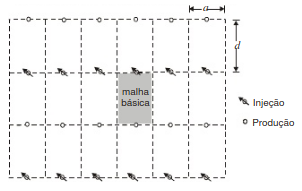
\includegraphics[width=.6\textwidth]{figs/revisao/revisao_injld.png}
\caption{Inje\c{c}\~{a}o em linha direta \cite[p. 567]{engres}.}
\label{fig:rev_injld}
\end{figure}

\begin{figure}[!ht]
\centering
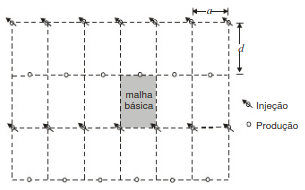
\includegraphics[width=.6\textwidth]{figs/revisao/revisao_injle.png}
\caption{Inje\c{c}\~{a}o em linhas esconsas \cite[p. 567]{engres}.}
\label{fig:rev_injle}
\end{figure}

Em alguns casos, os esquemas de malha em linhas diretas ou esconsas podem ser adaptados utilizando-se pol\'{i}gonos regulares como constituintes da malha; tr\^{e}s exemplos deste tipo de caso s\~{a}o:
\begin{itemize}
\item \textbf{Malha \textit{five-spot}:} Neste caso, a malha \'{e} formada por linhas esconsas, formando um quadrado perfeito; um po\c{c}o produtor \'{e} cercado por quatro injetores.
\item \textbf{Malha \textit{seven-spot}:} A malha considerada consiste em hex\'{a}gonos regulares, em que um po\c{c}o produtor \'{e} cercado por seis injetores; pode ser considerada um esquema de linhas esconsas, mas com altern\^{a}ncia de dois injetores para cada produtor em cada linha.
\item \textbf{Malha \textit{nine-spot}:} Assim como a malha \textit{five-spot}, \'{e} constitu\'{i}da por quadrados; por\'{e}m, o esquema de inje\c{c}\~{a}o base pode ser visto como linhas diretas, em que h\'{a} linhas s\'{o} de injetores e linhas alternadas entre produtores e injetores; neste tipo de malha, cada po\c{c}o produtor \'{e} cercado por oito po\c{c}os injetores.
\end{itemize}

Os esquemas de inje\c{c}\~{a}o em malhas vistos at\'{e} aqui consideram um po\c{c}o produtor cercado de v\'{a}rios injetores; s\~{a}o consideradas, portanto, malhas de tipo \textit{normal}. Contudo, as mesmas malhas podem tamb\'{e}m ser projetadas tomando-se em conta um po\c{c}o injetor cercado por v\'{a}rios produtores; s\~{a}o as chamadas \textit{malhas invertidas} ou \textit{inversas} \cite[p. 569]{engres}. A Figuras \ref{fig:rev_inj7i} mostra alguns exemplos de malhas de inje\c{c}\~{a}o, enquanto que a Tabela \ref{tab:wfdpat} destaca algumas informa\c{c}\~{o}es relativas aos esquemas de inje\c{c}\~{a}o vistos.

\begin{figure}[!ht]
\centering
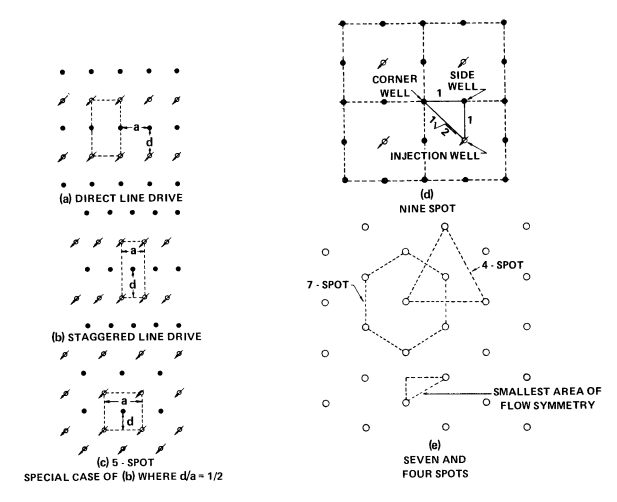
\includegraphics[width=.7\textwidth]{figs/revisao/revisao_injmalhas.png}
\caption{Exemplos de malhas de inje\c{c}\~{a}o \cite{singh1982}.}
\label{fig:rev_inj7i}
\end{figure}

\begin{table}[!ht]
	\centering
	\caption{Caracter\'{i}sticas de alguns esquemas de inje\c{c}\~{a}o, adaptado de \cite{singh1982}\label{tab:wfdpat}}
	\begin{tabular}{|c|c|c|}
		\hline
		\textbf{Esquema} & \textbf{Raz\~{a}o produtores/injetores} & \textbf{Padr\~{a}o de fura\c{c}\~{a}o} \\ \hline
		\textit{Four-spot} & $2$ & Tri\^{a}ngulo equil\'{a}tero \\ \hline
		\textit{Four-spot} obl\'{i}quo & $2$ & Quadrado \\ \hline
		\textit{Five-spot} & $1$ & Quadrado \\ \hline
		\textit{Seven-spot} & $\frac{1}{2}$ & Tri\^{a}ngulo equil\'{a}tero \\ \hline
		\textit{Seven-spot} invertido (injetor \'{u}nico) & $2$ & Tri\^{a}ngulo Equil\'{a}tero \\ \hline
		\textit{Nine-spot} & $\frac{1}{3}$ & Quadrado \\ \hline
		\textit{Nine-spot} invertido (injetor \'{u}nico) & $3$ & Quadrado \\ \hline
		Linhas diretas & $1$ & Ret\^{a}ngulo \\ \hline
		Linhas esconsas & $1$ & Linhas deslocadas \\ \hline
		
	\end{tabular}
\end{table}

Assim como no caso da inje\c{c}\~{a}o perif\'{e}rica, os esquemas de inje\c{c}\~{a}o em malhas possuem larga utiliza\c{c}\~{a}o na engenharia de reservat\'{o}rios; Zakirov \textit{et al.}, por exemplo, fazem a compara\c{c}\~{a}o de v\'{a}rios esquemas de malha no projeto de inje\c{c}\~{a}o de \'{a}gua no campo de Russkoye, situado acima do C\'{i}rculo Polar na R\'{u}ssia, com a an\'{a}lise feita em termos econ\^{o}micos e avalia\c{c}\~{a}o t\'{e}cnica \cite{zakirov2012}. Um outro uso \'{e} proposto por Zhou \textit{et al.}; por\'{e}m, neste caso os esquemas de inje\c{c}\~{a}o em malhas s\~{a}o testados em outros m\'{e}todos de recupera\c{c}\~{a}o, como a inje\c{c}\~{a}o de pol\'{i}meros e surfactantes \cite{zhou2016}.

\subsection{Aspectos Operacionais da Inje\c{c}\~{a}o de \'{A}gua}

O m\'{e}todo de recupera\c{c}\~{a}o secund\'{a}ria por inje\c{c}\~{a}o de \'{a}gua \'{e} ainda um dos mais utilizados; ela tem o objetivo de deslocar o \'{o}leo em dire\c{c}\~{a}o aos po\c{c}os produtores, aumentando assim a produ\c{c}\~{a}o de petr\'{o}leo em rela\c{c}\~{a}o \`{a} recupera\c{c}\~{a}o prim\'{a}ria.

A inje\c{c}\~{a}o de \'{a}gua no reservat\'{o}rio faz com que a satura\c{c}\~{a}o de \'{a}gua se eleve nas imedia\c{c}\~{o}es dos po\c{c}os injetores; esse aumento de satura\c{c}\~{a}o gera um banco de \'{o}leo cujo avan\c{c}o se d\'{a} em dire\c{c}\~{a}o aos po\c{c}os produtores. Uma vez alcan\c{c}ando esses po\c{c}os, o banco de \'{o}leo faz com que a produ\c{c}\~{a}o de \'{o}leo aumente bruscamente. 

Segundo Rosa, o per\'{i}odo de tempo entre o in\'{i}cio das opera\c{c}\~{o}es e a chegada do \'{o}leo ao po\c{c}o produtor \'{e} chamado de tempo de enchimento (\textit{``fill up''}); posteriormente, a frente de avan\c{c}o atinge o po\c{c}o produtor, aumentando bruscamente a raz\~{a}o \'{a}gua/\'{o}leo (RAO), ocorrendo ent\~{a}o o que se chama de erup\c{c}\~{a}o (\textit{``breakthrough''}). Ap\'{o}s a erup\c{c}\~{a}o, a RAO continua a crescer at\'{e} atingir n\'{i}veis que ir\~{a}o inviabilizar economicamente a produ\c{c}\~{a}o do po\c{c}o, o qual \'{e} fechado ou eventualmente transformado em po\c{c}o injetor \cite{engres}.

\subsubsection{Fatores de Influ\^{e}ncia}

Os projetos de inje\c{c}\~{a}o de \'{a}gua dependem n\~{a}o somente do objetivo de se obter uma melhor produ\c{c}\~{a}o de petr\'{o}leo; os fatores f\'{i}sicos do reservat\'{o}rio, por exemplo, tamb\'{e}m devem ser levados em conta na fase inicial do projeto. Os seguintes fatores ajudam a ditar par\^{a}metros de um projeto de inje\c{c}\~{a}o de \'{a}gua\footnote{Ver \cite[pp. 652-653]{engres}} (como formato da malha de inje\c{c}\~{a}o, n\'{u}mero de injetores, entre outros):

\begin{enumerate}
\item \textbf{Mecanismos de produ\c{c}\~{a}o do reservat\'{o}rio:} A depender do mecanismo de produ\c{c}\~{a}o, a quantidade de \'{a}gua a ser injetada varia; no caso de um influxo de \'{a}gua, por exemplo, ser\'{a} requerida uma menor vaz\~{a}o de inje\c{c}\~{a}o (ou essa vaz\~{a}o at\'{e} poder\'{a} ser nula) para que a press\~{a}o do reservat\'{o}rio seja mantida. O balan\c{c}o de materiais (diferen\c{c}a entre o volume que sai e o volume que \'{e} reposto pela natureza) ir\'{a} determinar o volume e a vaz\~{a}o total que dever\'{a} ser reposta pela recupera\c{c}\~{a}o secund\'{a}ria. J\'{a} no caso do mecanismo de g\'{a}s em solu\c{c}\~{a}o, a quantidade de \'{a}gua injetada deve ser maior, pois a press\~{a}o tende a cair rapidamente, ou seja, a deple\c{c}\~{a}o do reservat\'{o}rio \'{e} mais r\'{a}pida, acarretando urg\^{e}ncia na ado\c{c}\~{a}o da recupera\c{c}\~{a}o secund\'{a}ria.

\item \textbf{Caracter\'{i}sticas da rocha:} Caracter\'{i}sticas como permeabilidade, porosidade, presen\c{c}a de finos, a argila do reservat\'{o}rio e sua composi\c{c}\~{a}o qu\'{i}mica s\~{a}o determinantes em um projeto de inje\c{c}\~{a}o de \'{a}gua; de acordo com Eremin e Nazarova, por exemplo, caso haja uma incompatibilidade qu\'{i}mica entre a \'{a}gua injetada e o reservat\'{o}rio, haver\'{a} uma deposi\c{c}\~{a}o de sais que, consequentemente, afetam a pososidade e a permeabilidade do reservat\'{o}rio, reduzindo a recupera\c{c}\~{a}o de \'{o}leo nos po\c{c}os produtores \cite{eremin}.

\item \textbf{Caracter\'{i}sticas dos fluidos:} Assim como nas caracter\'{i}sticas da rocha, deve-se haver uma compatibilidade qu\'{i}mica entre a \'{a}gua injetada e os fluidos do reservat\'{o}rio, de maneira a evitar a forma\c{c}\~{a}o de precipitados; al\'{e}m disso, caso haja uma alta raz\~{a}o de mobilidades entre o \'{o}leo e a \'{a}gua, deve-se aumentar o n\'{u}mero de po\c{c}os injetores e diminuir a vaz\~{a}o dos mesmos, de maneira a evitar um \textit{``breakthrough''} prematuro nos po\c{c}os produtores.

\item \textbf{Profundidade do reservat\'{o}rio:} O gradiente m\'{a}ximo de press\~{a}o entre os po\c{c}os injetores e o reservat\'{o}rio \'{e} diretamente influenciado pela sua profundidade, por esta ser proporcional \`{a}s press\~{o}es de inje\c{c}\~{a}o e fraturamento do reservat\'{o}rio.

\item \textbf{Conforma\c{c}\~{a}o estrutural do reservat\'{o}rio:} A depender da estrutura do reservat\'{o}rio, torna-se preferencial a ado\c{c}\~{a}o de esquemas de inje\c{c}\~{a}o espec\'{i}ficos; o esquema de inje\c{c}\~{a}o perif\'{e}rica, por exemplo, \'{e} adequado para reservat\'{o}rios muito inclinados, onde a segrega\c{c}\~{a}o gravitacional dos fluidos \'{e} grande.
\end{enumerate}

Os fatores de influ\^{e}ncia, al\'{e}m de ditar o n\'{u}mero de injetores e a vaz\~{a}o de inje\c{c}\~{a}o, por exemplo, tamb\'{e}m s\~{a}o determinantes para a escolha do esquema de inje\c{c}\~{a}o a ser adotado, conforme afirma Stephens; o autor cita exemplos de reservat\'{o}rios em que, por exemplo, \'{e} invi\'{a}vel a ado\c{c}\~{a}o de projetos de inje\c{c}\~{a}o em malha, como o \textit{five-spot}, e outros em que n\~{a}o \'{e} recomendado o uso de inje\c{c}\~{a}o perif\'{e}rica; no seu trabalho, Stephens cita cinco exemplos de casos baseados em reservat\'{o}rios reais, discutindo qual o melhor esquema de inje\c{c}\~{a}o para os mesmos, considerando-se os par\^{a}metros dos reservat\'{o}rios \cite{stephens1960}.

\subsubsection{Componentes Principais de um Sistema de Inje\c{c}\~{a}o}

Vistos os fatores que influenciam um projeto de recupera\c{c}\~{a}o secund\'{a}ria por inje\c{c}\~{a}o de \'{a}gua, procede-se \`{a} descri\c{c}\~{a}o dos seus componentes principais\footnote{Ver \cite[pp. 653-659]{engres}}:

\begin{enumerate}
\item \textbf{Capta\c{c}\~{a}o:} A capta\c{c}\~{a}o do fluido injetado pode se dar de rios, lagos, mares, subsuperf\'{i}cie, \'{a}gua de produ\c{c}\~{a}o ou at\'{e} mesmo de outros campos de reservat\'{o}rios.

\item \textbf{Adu\c{c}\~{a}o:} Sistema de transporte \'{a}gua. Como lida com \'{a}gua n\~{a}o tratada, devem ser empregados materiais resistentes \`{a} agressividade da \'{a}gua para desenvolver esse sistemas. A redu\c{c}\~{a}o de dep\'{o}sitos s\'{o}lidos tamb\'{e}m deve ser considerada.

\item \textbf{Tancagem:} Sistema de armazenamento de \'{a}gua; a depender do tipo de capta\c{c}\~{a}o da \'{a}gua, a tancagem de \'{a}gua bruta pode ser largamente utilizada ou at\'{e} mesmo dispensada (como em casos de capta\c{c}\~{a}o da \'{a}gua do mar). A tancagem de \'{a}gua pot\'{a}vel, por outro lado, \'{e} necess\'{a}ria para armazenar reserva para determinados equipamentos, como por exempo, \'{a}gua limpa para contra-lavagem dos filtros ou para refrigera\c{c}\~{a}o de bombas.

\item \textbf{Tratamento:} A \'{a}gua bruta a ser utilizada precisa ser tratada, de maneira a ser propriamente injetada; os dois principais m\'{e}todos utilizados de tratamento s\~{a}o a retirada de s\'{o}lidos e o controle bacteriol\'{o}gico, j\'{a} que as bact\'{e}rias tendem a consumir o petr\'{o}leo, por este ser composto majoritariamente de mat\'{e}ria org\^{a}nica.

\item \textbf{Conjunto motor-bomba:} Respons\'{a}vel pelo fornecimento de energia para a \'{a}gua se deslocar em dire\c{c}\~{a}o ao reservat\'{o}rio com a vaz\~{a}o desejada. Dois tipos de bombas s\~{a}o normalmente utilizados: bombas centr\'{i}fugas, em sistemas de press\~{a}o mais baixa, e bombas alternativas (deslocamento positivo) em sistemas de alta press\~{a}o.

\item \textbf{Rede de distribui\c{c}\~{a}o:} Integra a esta\c{c}\~{a}o de inje\c{c}\~{a}o de \'{a}gua, um sistema adutor e os po\c{c}os de inje\c{c}\~{a}o. H\'{a} dois tipos, apresentados na Figura \ref{fig:rev_redis}: a rede de distribui\c{c}\~{a}o em marcha (``espinha de peixe'') e a centralizada atrav\'{e}s de \textit{``manifolds''} (``p\'{e} de galinha'').

\begin{figure}[!ht]
\centering
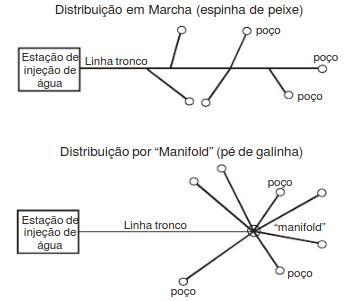
\includegraphics[width=.6\textwidth]{figs/revisao/revisao_redis.png}
\caption{Esquemas de redes de distribui\c{c}\~{a}o \cite[p. 657]{engres}.}\label{fig:rev_redis}
\end{figure}

\item \textbf{Po\c{c}os de inje\c{c}\~{a}o:} A maioria dos po\c{c}os injetores s\~{a}o, na verdade, antigos po\c{c}os produtores convertidos ou recompletados para inje\c{c}\~{a}o; h\'{a} at\'{e} mesmo casos em que o mesmo po\c{c}o comporta uma zona produtora e outra injetora. Alguns tipos de completa\c{c}\~{a}o de po\c{c}os injetores s\~{a}o apresentados na Figura \ref{fig:rev_incmp}. 

\begin{figure}[!ht]
\centering
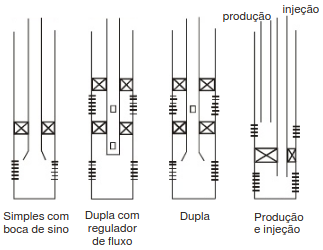
\includegraphics[width=.6\textwidth]{figs/revisao/revisao_injcomp.png}
\caption{Tipos de completa\c{c}\~{a}o de po\c{c}os de inje\c{c}\~{a}o de \'{a}gua \cite[p. 658]{engres}.}\label{fig:rev_incmp}
\end{figure}

\item \textbf{Po\c{c}os de capta\c{c}\~{a}o:} Normalmente, s\~{a}o antigos po\c{c}os produtores de \'{o}leo, recompletados (recanhoneados) em zonas produtoras de \'{a}gua. Apesar de serem po\c{c}os previamente abandonados, s\~{a}o po\c{c}os problem\'{a}ticos, devido \`{a}s altas vaz\~{o}es de fluido com sais dissolvidos, tais po\c{c}os produzem areia, diminuindo a vida \'{u}til dos equipamentos.

\item \textbf{Po\c{c}os de \textit{``dump-flood''}:} S\~{a}o os sistemas mais simples de inje\c{c}\~{a}o de \'{a}gua, consistindo simplesmente em po\c{c}os simultaneamente produtores e injetores de \'{a}gua, isto \'{e}, produzem \'{a}gua na zona superior e injetam diretamente, por gravidade, na zona inferior. A opera\c{c}\~{a}o desse tipo de po\c{c}o \'{e} muito simples, mas o acompanhamento somente \'{e} poss\'{i}vel atrav\'{e}s de perfilagens peri\'{o}dicas com o chamado
medidor de fluxo cont\'{i}nuo (\textit{``continuous flow meter''}) ou com perfilagem radiativa.
\end{enumerate}

\'{E} importante destacar a necessidade de se ter aten\c{c}\~{a}o \`{a}s caracter\'{i}sticas dos po\c{c}os de inje\c{c}\~{a}o projetados de maneira a se obter o desempenho \'{o}timo; Palsson \textit{et al.} citam algumas dessas caracter\'{i}sticas, como inclina\c{c}\~{a}o e orienta\c{c}\~{a}o dos po\c{c}os, completa\c{c}\~{a}o e danos de perfura\c{c}\~{a}o e completa\c{c}\~{a}o. Os desafios t\'{e}cnicos principais s\~{a}o:

\begin{itemize}
	\item Obter e manter a vaz\~{a}o de inje\c{c}\~{a}o desejada;
	\item Controlar o perfil de injetividade para a obten\c{c}\~{a}o da m\'{a}xima efici\^{e}ncia de varrido;
	\item Reduzir as incertezas na opera\c{c}\~{a}o esperada da inje\c{c}\~{a}o nos po\c{c}os.
\end{itemize}

Os autores ainda destacam a import\^{a}ncia da completa\c{c}\~{a}o dos po\c{c}os de inje\c{c}\~{a}o com o intuito dos mesmos suportarem altas press\~{o}es de inje\c{c}\~{a}o e diminuir custos de manuten\c{c}\~{a}o, como troca de tubos; al\'{e}m disso, s\~{a}o citados alguns problemas que podem surgir durante projetos de inje\c{c}\~{a}o, como o caso da perda de po\c{c}os devido ao entupimento com areia, consequ\^{e}ncia da presen\c{c}a de po\c{c}os injetores em forma\c{c}\~{o}es n\~{a}o consolidadas \cite{PALSSON2003333}. 

\subsubsection{Controle e Acompanhamento}
De maneira a se acompanhar satisfatoriamente um projeto de inje\c{c}\~{a}o de \'{a}gua, n\~{a}o se deve apenas controlar os valores de vaz\~{a}o, mantendo-as nas cotas estabelecidas; tal controle, segundo Rosa, seria suficiente se as forma\c{c}\~{o}es fossem homog\^{e}neas e as suas condi\c{c}\~{o}es de permeabilidade e press\~{a}o se mantivessem inalteradas ao longo do tempo. Sabe-se, contudo, que isso \'{e} praticamente imposs\'{i}vel de ocorrer, devendo-se portanto realizar testes peri\'{o}dicos para que possam ser identificadas situa-\c{c}\~{o}es indesejadas como, por exemplo, dano \`{a} forma\c{c}\~{a}o e m\'{a} distribui\c{c}\~{a}o da \'{a}gua. Algumas estrat\'{e}gias de controle e acompanhamento s\~{a}o apresentadas a seguir\footnote{Ver \cite[pp. 659-662]{engres}}:

\begin{enumerate}
\item \textbf{Testes:} H\'{a} v\'{a}rios tipos de testes para acompanhamento dos po\c{c}os de inje\c{c}\~{a}o de \'{a}gua; entre eles o teste de inje\c{c}\~{a}o, que busca acompanhar a vaz\~{a}o e a press\~{a}o de inje\c{c}\~{a}o, fornecendo uma primeira ideia do comportamento do po\c{c}o; o teste de \textit{fall-off}, que avalia se a forma\c{c}\~{a}o est\'{a} danificada, estimulada ou se est\'{a} em sua condi\c{c}\~{a}o original; e o teste \textit{step rate}, que, ao realizar a inje\c{c}\~{a}o com press\~{o}es variadas, obt\'{e}m valores distintos de vaz\~{o}es; com esses dados, \'{e} poss\'{i}vel construir um gr\'{a}fico da vaz\~{a}o em fun\c{c}\~{a}o da press\~{a}o, conforme ilustra a Figura \ref{fig:rev_tst}.

\begin{figure}[!ht]
\centering
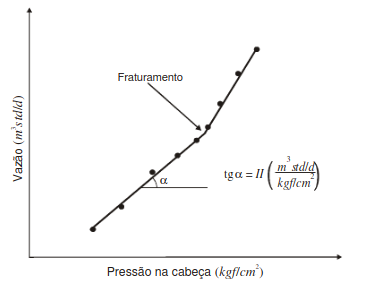
\includegraphics[width=.6\textwidth]{figs/revisao/revisao_tst.png}
\caption{Teste \textit{step rate} \cite[p. 660]{engres}.}\label{fig:rev_tst}
\end{figure}

\item \textbf{\'{I}ndice de injetividade:} Similar ao \'{i}ndice de produtividade para po\c{c}os produtores, esse \'{i}ndice pode indicar, se calculado periodicamente, a causa do decr\'{e}scimo de vaz\~{a}o durante os primeiros est\'{a}gios de inje\c{c}\~{a}o de um po\c{c}o; esse \'{i}ndice pode ser estimado a partir de testes de inje\c{c}\~{a}o, \textit{fall-off} ou \textit{step rate}.

\item \textbf{Perfil de Injetividade:} Destina-se \`{a} investiga\c{c}\~{a}o da distribui\c{c}\~{a}o de \'{a}gua atrav\'{e}s da forma\c{c}\~{a}o, uma vez que a presen\c{c}a de fraturas naturais ou induzidas, zonas de alta permeabilidade devidas \`{a} heterogeneidade do reservat\'{o}rio, etc., podem provocar uma erup\c{c}\~{a}o precoce de \'{a}gua de inje\c{c}\~{a}o nos po\c{c}os produtores, prejudicando a efici\^{e}ncia de varrido e, consequentemente, a produ\c{c}\~{a}o. Deste modo, com a corre\c{c}\~{a}o de eventuais anomalias, consegue-se aumentar a recupera\c{c}\~{a}o de \'{o}leo e reduzir a produ\c{c}\~{a}o de \'{a}gua, logo reduzindo-se os gastos com tratamento qu\'{i}mico, principalmente.
\end{enumerate} 

O processo de controle e acompanhamento de projetos de inje\c{c}\~{a}o de \'{a}gua se econtra bem difundido na literatura; Talash, por exemplo, afirma que um fator essencial para o sucesso de um projeto de inje\c{c}\~{a}o de \'{a}gua envolve um programa de controle e acompanhamento bem planejados e executados\footnote{O autor destaca m\'{e}todos de acompanhamento n\~{a}o s\'{o} do projeto de inje\c{c}\~{a}o, como o de reservat\'{o}rios e tamb\'{e}m dos componentes; ver \cite{talash1988}.}. J\'{a} Palsson \textit{et al.} consideram que o monitoramento da injetividade de \'{a}gua \'{e} comumente limitado a medidas de press\~{a}o e vaz\~{a}o em intervalos de tempo regulares; os autores citam algumas formas de apresenta\c{c}\~{a}o dos dados, como curvas de press\~{a}o/vaz\~{a}o, curvas de press\~{a}o e vaz\~{a}o em fun\c{c}\~{a}o do tempo, diagrama de Hall, entre outros; al\'{e}m disso, afirmam que essas representa\c{c}\~{o}es podem identificar mudan\c{c}as na injetividade dos po\c{c}os \cite{PALSSON2003333}.

\subsubsection{Principais Problemas}
Alguns dos principais problemas envolvendo a inje\c{c}\~{a}o de \'{a}gua s\~{a}o relacionados, al\'{e}m do aspecto econ\^{o}mico, tamb\'{e}m aos aspectos f\'{i}sico-qu\'{i}micos do fluido injetado e do reservat\'{o}rio. Um problema not\'{a}vel \'{e} a corros\~{a}o met\'{a}lica em sistemas de inje\c{c}\~{a}o, particularmente em casos de \'{a}guas com elevada salinidade e gases dissolvidos como oxig\^{e}nio, sulfeto de hidrog\^{e}nio e di\'{o}xido de carbono. Rosa apresenta alguns efeitos f\'{i}sicos-qu\'{i}micos diretamente relacionados ao fen\^{o}meno da corros\~{a}o met\'{a}lica \cite[pp. 662-663]{engres}:

\begin{enumerate}
\item \textbf{Efeitos da composi\c{c}\~{a}o da \'{a}gua:} Al\'{e}m da presen\c{c}a de gases dissolvidos ser um importante fator na corros\~{a}o met\'{a}lica, a pr\'{o}pria condutividade da \'{a}gua \'{e} diretamente proporcional \`{a} sua corrosividade.

\item \textbf{Efeitos de vari\'{a}veis f\'{i}sicas:} A temperatura, a press\~{a}o e a velocidade da \'{a}gua s\~{a}o fatores determinantes para sua corrosividade; a temperatura, por exemplo, aumenta drasticamente a corros\~{a}o quando elevada em sistemas fechados. Por\'{e}m, em sistemas abertos, a corros\~{a}o aumenta com a temperatura aumenta at\'{e} certo ponto, passando a diminuir por conta da libera\c{c}\~{a}o r\'{a}pida dos gases dissolvidos. A press\~{a}o \'{e} determinante para alterar rea\c{c}\~{o}es qu\'{i}micas; nos sistemas de inje\c{c}\~{a}o de \'{a}gua, ela influi diretamente na solubilidade dos gases em solu\c{c}\~{a}o, variando a taxa de corros\~{a}o. Por fim, a velocidade da \'{a}gua, ao ser elevada, acarreta em uma taxa de corros\~{a}o maior; por\'{e}m, \'{a}guas paradas ou de baixa vaz\~{a}o podem provocar a decanta\c{c}\~{a}o de s\'{o}lidos em suspens\~{a}o nos equipamentos de inje\c{c}\~{a}o.
\end{enumerate}

Um outro problema relevante em sistemas de inje\c{c}\~{a}o de \'{a}gua tem a ver com a forma\c{c}\~{a}o, devido aos componentes dissolvidos na \'{a}gua e outros fatores, de dep\'{o}sitos salinos nos equipamentos. Em quase todas as \'{a}guas, por exemplo, h\'{a} a presen\c{c}a de sais de c\'{a}lcio e magn\'{e}sio, cuja deposi\c{c}\~{a}o \'{e} a menos danosa, por ser facilmente remediada. J\'{a} a presen\c{c}a de compostos ferrosos conduzem \`{a} corros\~{a}o galv\^{a}nica; a presen\c{c}a de sulfetos \'{e} a mais danosa, pois, al\'{e}m da corros\~{a}o, provoca abras\~{a}o por atrito nas tubula\c{c}\~{o}es. Um outro efeito danoso dos sulfetos \'{e} a ocorr\^{e}ncia de s\'{e}rios danos \`{a} forma\c{c}\~{a}o, podendo ocasionar o tamponamento total da mesma.

Outros tipos de sais que se depositam nos sistemas de inje\c{c}\~{a}o de \'{a}gua e reservat\'{o}rios s\~{a}o os sais de b\'{a}rio. Estes causam danos \`{a} forma\c{c}\~{a}o irrevers\'{i}veis, pois o sulfato de b\'{a}rio, por exemplo, \'{e} insol\'{u}vel em \'{a}cidos, que normalmente s\~{a}o utilizados para lidar com dep\'{o}sitos salinos; neste caso, uma das medidas para evitar essa deposi\c{c}\~{a}o \'{e} impedir a forma\c{c}\~{a}o do sulfato de b\'{a}rio a partir do uso de inibidores qu\'{i}micos. Por fim, outro tipo de deposi\c{c}\~{a}o em sistemas de inje\c{c}\~{a}o \'{e} a s\'{i}lica, que, al\'{e}m de formar deposi\c{c}\~{o}es, pode auxiliar no tamponamento de linhas por outros precipitados ou at\'{e} mesmo ser aglutinada pelo \'{o}leo residual da \'{a}gua produzida. Neste caso, \'{e} empregado \'{a}cido fluor\'{i}drico para dissolv\^{e}-la\footnote{Todos esses problemas de deposi\c{c}\~{a}o de sais s\~{a}o explicados em \cite[p. 664]{engres}.}.

Outro problema a ser considerado considerando-se os fatores qu\'{i}micos envolvidos na inje\c{c}\~{a}o de \'{a}gua \'{e} a forma\c{c}\~{a}o de l\^{a}minas salinas nos tubos; segundo Adeniyi \textit{et al.}, esse fato acontece geralmente com a inje\c{c}\~{a}o de \'{a}gua n\~{a}o compat\'{i}vel com o reservat\'{o}rio, como por exemplo a inje\c{c}\~{a}o de \'{a}gua do mar em forma\c{c}\~{o}es ricas em \'{i}ons de estr\^{o}ncio e b\'{a}rio. Os autores citam os seguintes problemas potenciais\footnote{Ver \cite{adeniyi2008}}:

\begin{enumerate}
	\item O ato de elevar e tratar a \'{a}gua de inje\c{c}\~{a}o pode causar problemas uma vez que a \'{a}gua injetada se torna inst\'{a}vel, gerando um problema cont\'{i}nuo;
	\item Injetar uma \'{a}gua est\'{a}vel, por\'{e}m incompat\'{i}vel com o reservat\'{o}rio em um novo po\c{c}o injetor tamb\'{e}m pode causar a forma\c{c}\~{a}o de l\^{a}minas. Esse problema diminui gradativamente com a lavagem completa do po\c{c}o com a \'{a}gua de inje\c{c}\~{a}o.
\end{enumerate}

Al\'{e}m do problema da deposi\c{c}\~{a}o de l\^{a}minas salinas, Adeniyi \textit{et al.} tamb\'{e}m tratam do problema da corros\~{a}o; os autores afirmam que as principais causas de corros\~{a}o envolvem destrui\c{c}\~{a}o de ferro, e que esse problema \'{e} o que mais afeta, de maneira adversa, a produ\c{c}\~{a}o, o transporte e o refino; tal fato ocorre com a presen\c{c}a impurezas que geram c\'{e}lulas eletrol\'{i}ticas, aumentando a possibilidade de corros\~{a}o; a substitui\c{c}\~{a}o dessas impurezas por carbono, no processo de fabria\c{c}\~{a}o do a\c{c}o, \'{e} um modo de controlar esse problema \cite{adeniyi2008}.